\documentclass[final,t,overlay]{beamer}
\mode<presentation>
{
  \usetheme{UCL}
}
\usepackage[size=a0,scale=1,debug]{beamerposter}

% additional packages
\usepackage[english]{babel}
\usepackage[utf8]{inputenc}
\usepackage{pstool}
\usepackage{calc}
\usepackage{import}
\usepackage{color}
\usepackage{multicol}
\usepackage{graphicx}
\usepackage{tikz}
\usepackage{amsmath}
\usepackage{amsthm,amsthm}
\usepackage{amssymb}
\usetikzlibrary{arrows,shapes}
\tikzstyle{square}=[draw, minimum size=2.5em]
\tikzstyle{round}=[draw,circle, minimum size=2.5em]

 \def\mm#1{\ensuremath{\boldsymbol{#1}}} % version: amsmath
 
\DeclareMathOperator{\diag}{diag}
\DeclareMathOperator{\var}{var}
\DeclareMathOperator{\med}{Median}
\DeclareMathOperator{\chol}{cholesky}
\DeclareMathOperator{\tr}{tr}
\DeclareMathOperator*{\minimise}{minimise}
\DeclareMathOperator*{\argmax}{arg\,max}
\DeclareMathOperator*{\argmin}{arg\,min}

\global\long\def\Mz{M_{\mathbf{z},y}}
\global\long\def\muz{\mu_{\mathbf{z}}}
\global\long\def\aj{\alpha^{(j)}}
\global\long\def\ajt{\left(\alpha^{(j)}\right)^{\top}}

%empf is red now
%\renewcommand{\emph}[1]{{\color{red}{#1}}}

\title{A Kernel Test of Goodness of Fit}
\author[SHORTAUTHOR]
{Kacper Chwialkowski$^*$ Heiko Strathmann$^*$ Arthur Gretton}
\institute[SHORTINSTITUTE]{Gatsby Unit, University College London.}

\date[SHORTDATE]{DATE}

\global\long\def\ev{\mathbb{E}}

\newtheorem{thm}{Theorem}
\definecolor{mg}{rgb}{0,0.44,0}
\usepackage{graphicx}

%\usepackage{placeins}
\begin{document}
\begin{frame}
\begin{columns}
\begin{column}{.33\linewidth}
%\vspace{-0.75cm}
\begin{block}{Motivating example: testing output of approximate MCMC}
\begin{minipage}{.49\linewidth}

\begin{align*}
 \theta_{1}&\sim{\cal N}(0,10);\theta_{2}\sim{\cal N}(0,1) \\
 X_{i} &\sim\frac{1}{2}{\cal N}(\theta_{1},4)+\frac{1}{2}{\cal N}(\theta_{1}+\theta_{2},4)
\end{align*}
 \vspace{1cm} 

%AG: changed text

MCMC: samples from distributions where normalization can't be computed.
Recent work on MCMC  incorporates tradeoff between bias/accuracy, e.g. \cite{korattikara2013austerity}.
%And so we turn the Bayesian Crank  to  obtain samples form the posteriori distribution. It obviously matters which matter which method we use, since quality of sample depends on it. 
\end{minipage}
\begin{minipage}{.4\linewidth}
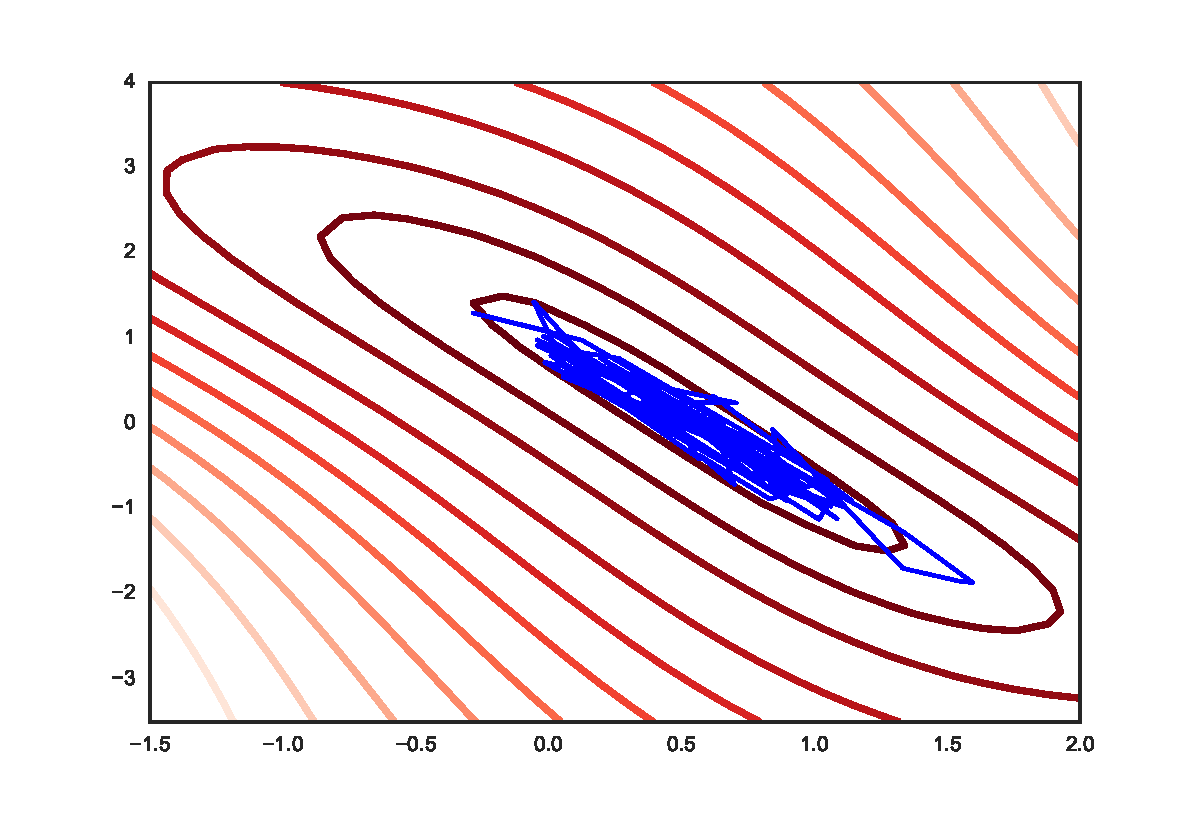
\includegraphics[scale=0.65]{../../presentation/img/sgld_trace_and_density.pdf}
\end{minipage}
\vspace{1cm}
\begin{center}
{\large\emph{How to check if MCMC samples match target distribution?}}
\end{center}
\end{block}
\vspace{-0.75cm}
\begin{block}{Maximum Mean Discrepancy for comparing two samples}
Maximum mean discrepancy: norm of function in RKHS revealing difference in distributions, \cite{gretton2012kernel}.

{\large\begin{align*}
MMD({\color{red} p},{ \color{blue} q},\mathcal{F}) = \sup_{   \| {\color{mg}f} \|_\mathcal{F}<1} [\ev_{{ \color{blue} q}}{\color{mg}f}- \ev_{{\color{red} p}}{\color{mg} f}]   
\end{align*}}
\begin{minipage}{.60\linewidth}

\vspace{1cm}

\normalsize
\vspace{1cm}
 \begin{itemize}
  \item $\mathcal{F}$ -- reproducing kernel Hilbert space.
  \item ${\color{mg} f^*}$ -- function that attains the supremum.
  \item We want to get rid of  $\ev_{ {\color{red} p} }f$ (usually can't compute in closed form)..
 \end{itemize}

\end{minipage}
\begin{minipage}{.35\linewidth}

\begin{center}
\vspace{-1cm}
\hspace{-2.5cm}
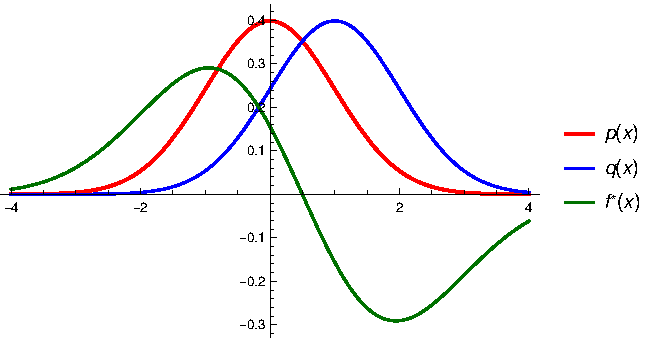
\includegraphics[scale=1.0]{../../presentation/img/mmd.pdf}
\end{center}
\end{minipage}
\vspace{1cm}
\begin{center}
{\large\emph{Can we do this without sampling from ${\color{red} p}$?}}
\end{center}
\end{block}
\vspace{-0.75cm}  %%%%%%%%%%%%%%%%%%%%%%%%%%%%%%%%%%%%%%%%%%%%%%%%%%%%%%%%%%%%
\begin{block}{Stein's trick in the RKHS}

%AG: fixed errors in proof

Consider the  class \large
$$G = \{ f'  +  \log' { \color{red} p} \cdot  f | f \in \mathcal{F} \}$$
\normalsize
Given $g\in G$, then (integration by parts)
\begin{align*}
\ev_{\color{red} p} g(X) &=
\ev_{\color{red} p} \left[ f'(X)  +  \log' {\color{red} p}(X) f(X) \right] \\
&= \int   f(x)' { \color{red} p}(x)   + f(x){\color{red} p}'(x) dx \\
&= \int_{-\infty}^{\infty} (f(x) {\color{red} p}(x) )'  dx \\
&= f(x) {\color{red} p}(x)  \big|_{x=-\infty}^{x=\infty} \\
&= 0
\end{align*}
Define the {\bf Stein operator}
\[
 T_{\color{red} p}f =  f'  +  \log' { \color{red} p} \cdot  f
\]
the function class is $G = \{ T_{\color{red} p}f | f \in \mathcal{F} \}$.

Inspired by \cite{gorham2015measuring}, related to \cite{OatGirCho15}, and independently developed in \cite{LiuLeeJor16}.
\end{block} %%%%%%%%%%%%%%%%%%%%%%%%%%%%%%%%%%%%%%%%%%%%%%%%%%%%%%%%%%%%
\vspace{-0.75cm}


\begin{block}{Maximum Stein discrepancy}
\large
\begin{align*}
MSD({\color{red} p},{ \color{blue} q},G) = \sup_{   \| {\color{mg} f} \|_\mathcal{F}<1} \ev_{{ \color{blue} q}} T_{\color{red} p} {\color{mg} f} - \ev_{{\color{red} p}} T_{\color{red} p} {\color{mg} f}  = \sup_{ \| {\color{mg} f} \|_\mathcal{F}<1} \ev_{{ \color{blue} q}} T_{\color{red} p} {\color{mg} f} 
\end{align*}
\vspace{2cm}
\centering
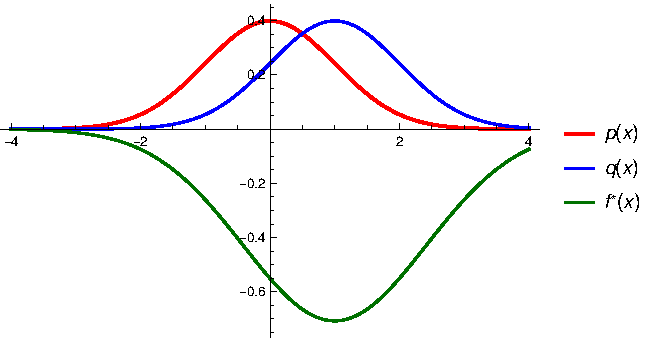
\includegraphics[scale=1.2]{../../presentation/img/s1.pdf}
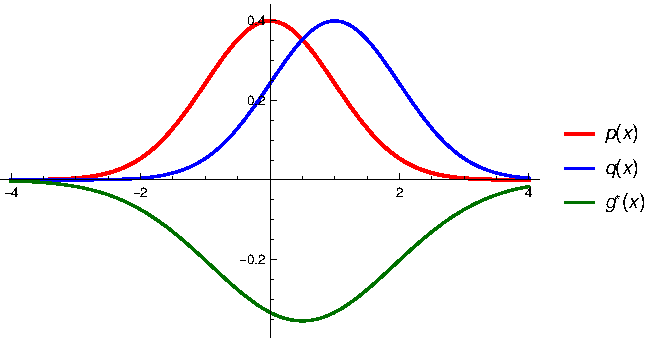
\includegraphics[scale=1.2]{../../presentation/img/s05.pdf}\\
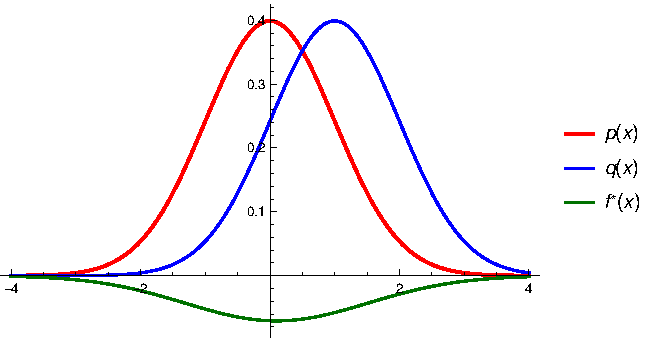
\includegraphics[scale=1.2]{../../presentation/img/s01.pdf}
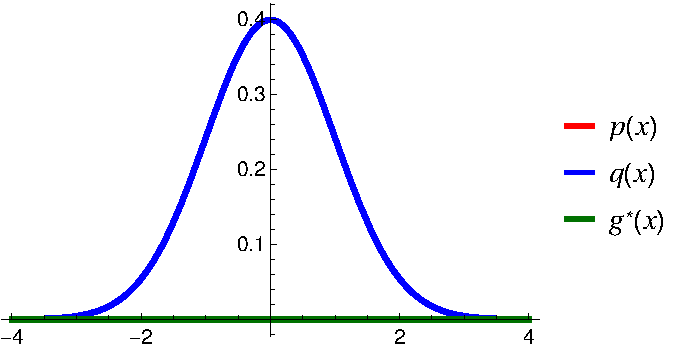
\includegraphics[scale=1.2]{../../presentation/img/s0.pdf}
\vspace{1cm}
\begin{center}
\emph{As { \color{blue} q} approaches {\color{red} p}, the {\color{mg} witness function} goes to 0. }
\end{center}
\end{block} %%%%%%%%%%%%%%%%%%%%%%%%%%%%%%%%%%%%%%%%%%%%%%%%%%%%%%%%%%%%


\vspace{-0.75cm}
\begin{block}{RKHS element for Stein operator}
%\Large
Given $f\in \mathcal{F}$, action of Stein operator $T_{\color{red} p}$ can be written as dot product with Stein element $\xi_{{ \color{red} p}}$,
 \begin{equation*}
T_{\color{red} p}[f](x) = \langle f, \xi_{{ \color{red} p}}(x,\cdot) \rangle_{\mathcal{F}}
\end{equation*}
where
 \begin{equation*}
\xi_{{ \color{red} p}}(x,\cdot):=\log' { \color{red} p}(x) k(x,\cdot)+  k'(x,\cdot).
\end{equation*}
and $k$ is kernel associated with RKHS $\mathcal{F}$.

%\large
Define $h_{{ \color{red} p}}$ as dot product of  $\xi$ at points $x$ and $y$, 
\[
h_{{\color{red} p}}(x,y)   = \langle\xi_{{ \color{red} p}}(x,\cdot),\xi_{{ \color{red} p}}(y,\cdot)\rangle. 
\]
$h_{{ \color{red} p}}$ can be written in closed form,
%\large
\begin{align*}
h_{{\color{red} p}}(x,y) & = \partial_{x} \log {\color{red} p}(x) \partial_{x} \log {\color{red} p}(y) k(x,y)\\
 & \quad+\partial_{y} \log {\color{red} p}(y) \partial_{x}  k(x,y)\\
 & \quad+\partial_{x} \log {\color{red} p}(x) \partial_{y}k(x,y)\\
 & \quad+\partial_{x} \partial_{y} k(x,y).
\end{align*}

\vspace{0.5cm}
\center{{\bf\emph{Only depends on kernel and $\partial_{x} \log {\color{red} p}(x)$, \\ do not need
to normalise {\color{red} p}, or sample from it. }}}
\end{block}

\vspace{-0.75cm}



 


\end{column}

%%%-----------------column 2
\hspace{-1.45cm}
\begin{column}{.33\linewidth}


\begin{block}{Theorem}
\large
Let ${ \color{blue} q},{\color{red} p}$ be probability measures and ${ \color{blue} Z}\sim { \color{blue} q}$. 
If $\ev_{{ \color{blue} q}} h_{{\color{red} p}}({ \color{blue} Z},{ \color{blue} Z})<\infty$, then 
$MSD({\color{red} p},{ \color{blue} q},G) = \ev_{{ \color{blue} q}} h_{{\color{red} p}}({ \color{blue} Z},{ \color{blue} Z}')$,
where ${ \color{blue} Z}'$ is an independent copy of ${ \color{blue} Z}$.
\end{block}

\vspace{-0.73cm}
\begin{block}{Proof}

First show that $\xi_{{ \color{red} p}}(x,\cdot)$ is Bochner integrable
\[
\ev_{{ \color{blue} q}}\|\xi_{{ \color{red} p}}({ \color{blue} Z})\|_{\mathcal{\mathcal{F}}}^{2}=\ev_{{ \color{blue} q}}h_{{ \color{red} p}}({ \color{blue} Z},{ \color{blue} Z})<\infty.
\]
We next relate the expected value of the Stein operator to the inner product of $f$ and the expected value
of $\xi_{{ \color{red} p}}({ \color{blue} Z})$,  
\begin{align*}
  \left\langle f,\ev_{{ \color{blue} q}} \xi_{{ \color{red} p}}({ \color{blue} Z}) \right\rangle _{\mathcal{\mathcal{F}}}& =\left\langle f,\ev_{{ \color{blue} q}} \left[  \log' { \color{red} p}({ \color{blue} Z}) k({ \color{blue} Z},\cdot)+\ k'({ \color{blue} Z},\cdot) \right] \right \rangle _{\mathcal{\mathcal{F}}}\\
 & = \ev_{{ \color{blue} q}}  \left\langle f,\left[  \log' { \color{red} p}({ \color{blue} Z}) k({ \color{blue} Z},\cdot)+\ k'({ \color{blue} Z},\cdot) \right] \right \rangle _{\mathcal{\mathcal{F}}}\\
 & =\ev_{{ \color{blue} q}}(T_{{ \color{red} p}}f)({ \color{blue} Z}).
\end{align*}
The second equality follows from  Bochner integrability of $\xi_{{ \color{red} p}}$.
We have 
\begin{align*}
MSD({ \color{red} p},{ \color{blue} q},G) & :=\sup_{\Vert f\Vert<1}\ev_{{ \color{blue} q}}(T_{{ \color{red} p}}f)({ \color{blue} Z})-\ev_{{ \color{red} p}}(T_{{ \color{red} p}}f)(X)\\
 & =\sup_{\Vert f\Vert<1}\ev_{{ \color{blue} q}}(T_{{ \color{red} p}}f)({ \color{blue} Z})\\
 & =\sup_{\Vert f\Vert<1}\langle f,\ev_{{ \color{blue} q}}\xi_{{ \color{red} p}}({ \color{blue} Z})\rangle_{{\cal \mathcal{F}}}\\
 & =\|\ev_{{ \color{blue} q}}\xi_{{ \color{red} p}}({ \color{blue} Z})\|_{\mathcal{\mathcal{F}}}.
\end{align*}
We now calculate closed form formula for $MSD({ \color{red} p},{ \color{blue} q},G)^{2}$,
\begin{align*}
MSD({ \color{red} p},{ \color{blue} q},G)^{2}  =\ev_{{ \color{blue} q}}\langle\xi_{{ \color{red} p}}({ \color{blue} Z}),\xi_{{ \color{red} p}}({ \color{blue} Z}')\rangle_{\mathcal{\mathcal{F}}}=\ev_{{ \color{blue} q}}h_{{ \color{red} p}}({ \color{blue} Z},{ \color{blue} Z}'),
\end{align*}
\end{block}


\vspace{-0.75cm}
\begin{block}{Theorem}
\vspace{1cm}


\large
If the kernel $k$ is $C_0$-universal, $\ev_{{ \color{blue} { \color{blue} q}}} h_{{ \color{blue} { \color{blue} q}}}({ \color{blue} Z},{ \color{blue} Z})<\infty$ and $\ev_{{ \color{blue} { \color{blue} q}}} (\log' \frac{{\color{red} p}({ \color{blue} Z})}{{ \color{blue} q}({ \color{blue} Z})})^{2}<\infty$
then $MSD({\color{red} p},{ \color{blue} q},G) =0$ if and only if ${\color{red} p}={ \color{blue} q}$.

\vspace{1cm}
\normalsize
Remarks.\\
Kernel is $C_0$-universal if  $f \to \int_X f(x) k(x,\cdot) d\mu(x)$ if is injective for all probability measures $\mu$ and all  $f \in L^p(X,\mu)$, where  $p \in [1,\infty] $. 
\vspace{0.5cm}

The assumption $\ev_{{ \color{blue} q}} (\log' \frac{{\color{red} p}({ \color{blue} Z})}{{ \color{blue} q}({ \color{blue} Z})})^{2}<\infty$ states that difference between scores $\log' \color{red} p$ and $\log' \color{blue} q$  is square integrable.
\end{block}

\vspace{-0.75cm}
\begin{block}{Proof}
 If ${ \color{red} p}={ \color{blue} q}$ then $MSD({\color{red} p},{ \color{red} p},G) =0$ is $0$. Suppose
${ \color{red} p}\neq { \color{blue} q}$, but $MSD({\color{red} p},{ \color{blue} q},G) =0$. If $MSD({\color{red} p},{ \color{blue} q},G) =0$ then, by Theorem 1 
$\ev_{{ \color{blue} q}}\xi_{{ \color{red} p}}({ \color{blue} Z})=0$. We substitute $\log { \color{red} p}({ \color{blue} Z})=\log { \color{blue} q}(Y)+[\log { \color{red} p}({ \color{blue} Z})-\log { \color{blue} q}(Y)]$,
\begin{align*}
 & \ev_{{ \color{blue} q}}\xi_{{ \color{red} p}}({ \color{blue} Z})\\
 & =\ev_{{ \color{blue} q}}\left( \log' { \color{red} p}({ \color{blue} Z})k({ \color{blue} Z},\cdot)+ k'({ \color{blue} Z},\cdot)\right)\\
 & =\ev_{{ \color{blue} q}}\xi_{{ \color{blue} q}}({ \color{blue} Z})+\ev_{{ \color{blue} q}}\left([\log { \color{red} p}({ \color{blue} Z})-\log { \color{blue} q}(Y)]'k({ \color{blue} Z},\cdot)\right)\\
 & =\ev_{{ \color{blue} q}}\left( [\log { \color{red} p}({ \color{blue} Z})-\log { \color{blue} q}(Y)]' k({ \color{blue} Z},\cdot)\right)
\end{align*}
The expected value of $(\log { \color{red} p}({ \color{blue} Z})-\log { \color{blue} q}({ \color{blue} Z}))' k({ \color{blue} Z},\cdot)$ is the mean embedding of
a function $g(y)=\left(\log\frac{{ \color{red} p}(y)}{{ \color{blue} q}(y)}\right)'$ with respect
to the measure ${ \color{blue} q}$.  $g$ is square integrable,
therefore, since the kernel $k$ is $C_0$-universal, %by \citet[ Theorem 4.4 c]{carmeli2010vector}
its embedding is zero if and only if $g=0$. This implies that 
\[
\log'\frac{{ \color{red} p}(y)}{{ \color{blue} q}(y)}=(0,\cdots,0).
\]
Consequently  $\log\frac{{ \color{red} p}(y)}{{ \color{blue} q}(y)}=C$, for some $C$, and so  ${ \color{red} p}(y)=e^{C}{ \color{blue} q}(y)$. Since ${ \color{red} p}$ and ${ \color{blue} q}$ both integrate
to one, $C=0$ then ${ \color{red} p}={ \color{blue} q}$, which is a contradiction.
\end{block}

\vspace{-0.75cm}
\begin{block}{Non i.i.d.\ extension: the wild bootstrap}
An estimator of $\ev_{\color{red} p} h_{\color{red} p}(X,X')$ is  
\[
 V_n(h_{\color{red} p}) = \frac {1} {n^2} \sum_{i,j=1}^n h_{\color{red} p}(X_i,X_j).
\]
To estimate quantiles of $ V_n(h_{\color{red} p})$ we use wild bootstrap
\[
 B_n(h_{\color{red} p}) = \frac {1} {n^2} \sum_{i,j=1}^n W_i W_j h_{\color{red} p}(X_i,X_j).
\]
  where $W_i$ is a  series  random variables.
\begin{center}
  \begin{minipage}{.49\linewidth}
       $$
  Cov(W_i,W_j) = (1-2p_n)^{-|i-j|}
  $$
\end{minipage}
\begin{minipage}{.49\linewidth}
 \begin{figure}
            \vspace{-0.5cm}
           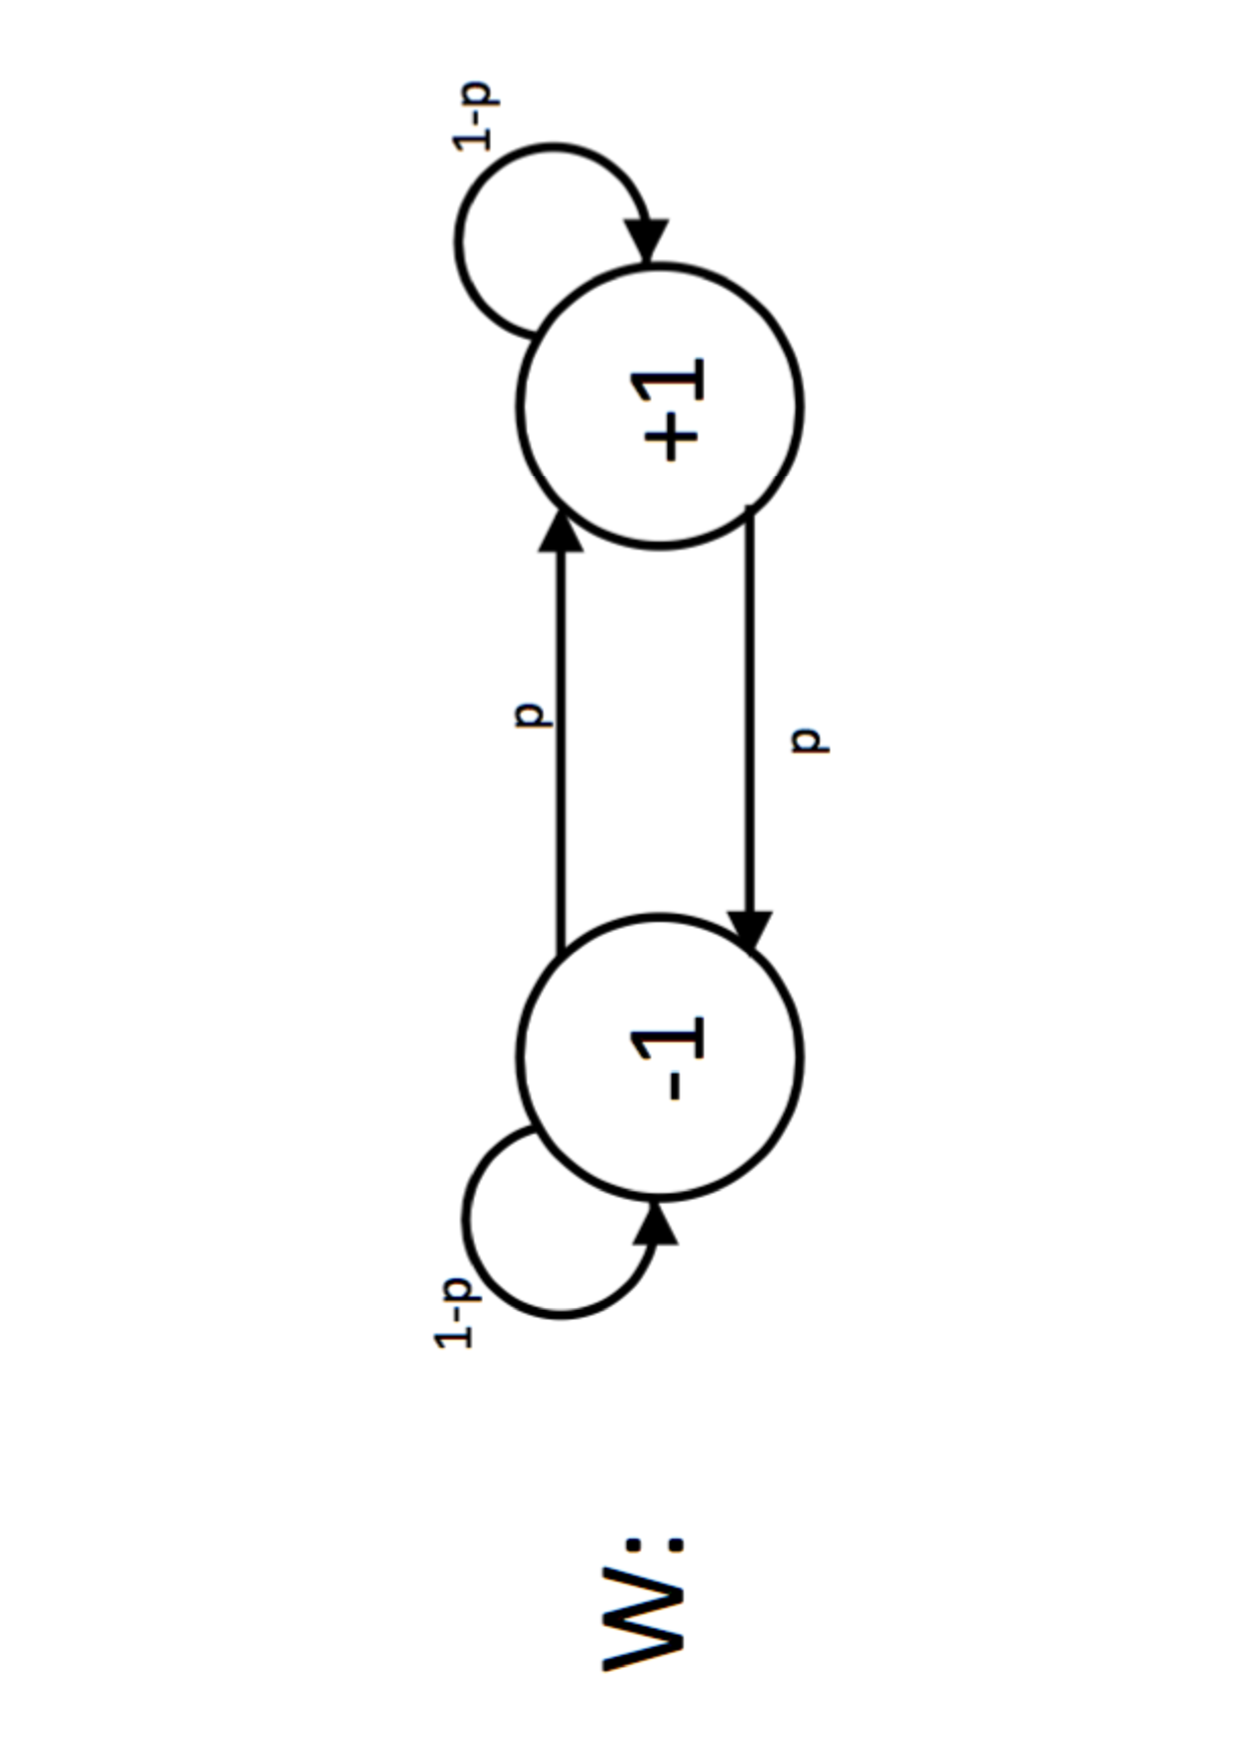
\includegraphics[width=0.7\textwidth, angle =0 ]{../../presentation/img/W_graphicalModel.pdf} 
        \end{figure}
\end{minipage}
\end{center}
  $p_n$ is  the probability of the change  and should be set to $o(n)$.

\setbeamertemplate{caption}{\raggedright\insertcaption\par}
\begin{center}

  \begin{minipage}{.49\linewidth}
\begin{figure}
 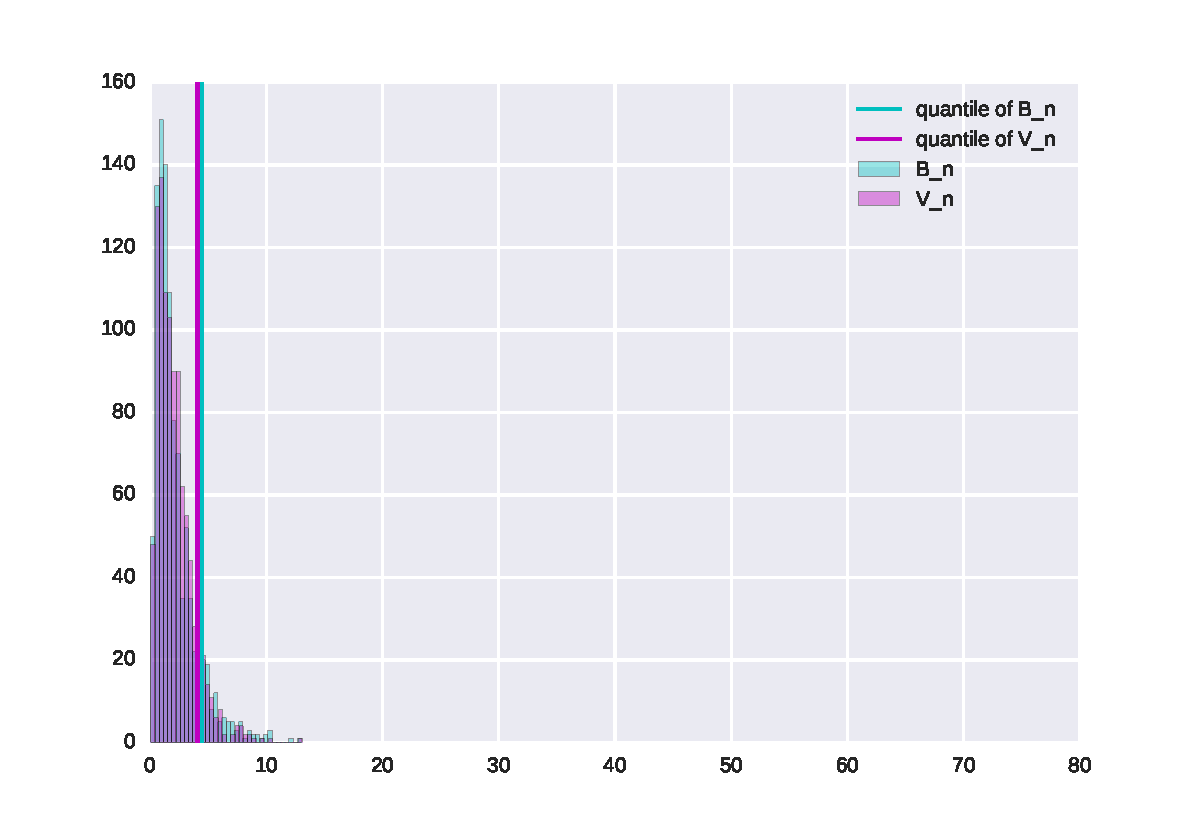
\includegraphics[width=\textwidth]{../../presentation/img/bootstrapWorks1.pdf}
 \caption{Small correlation in $W_t$} 
\end{figure}
 \end{minipage}
  \begin{minipage}{.49\linewidth}
\begin{figure}
 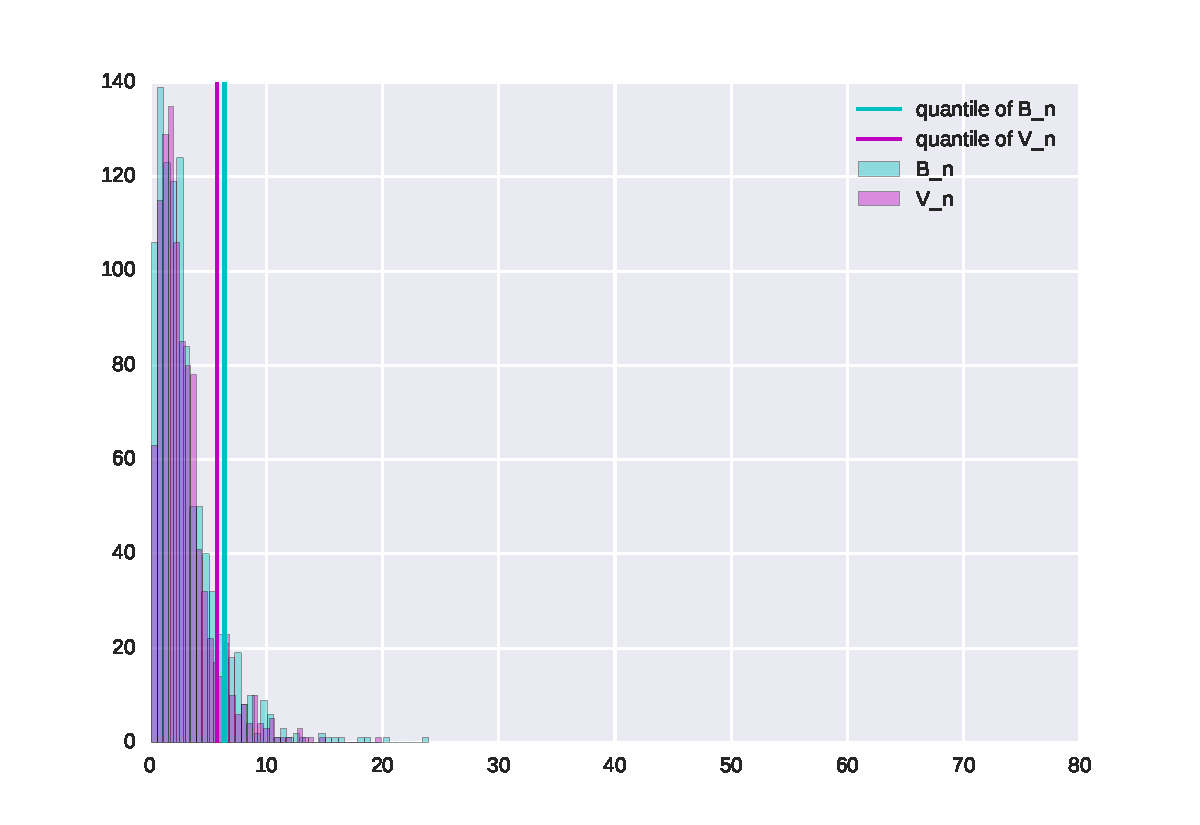
\includegraphics[width=\textwidth]{../../presentation/img/bootstrapWorks4.pdf}
 \caption{Medium correlation in $W_t$} 
\end{figure}
  \end{minipage}
\end{center}




 \begin{center}
  \begin{minipage}{.49\linewidth}
\begin{figure}
 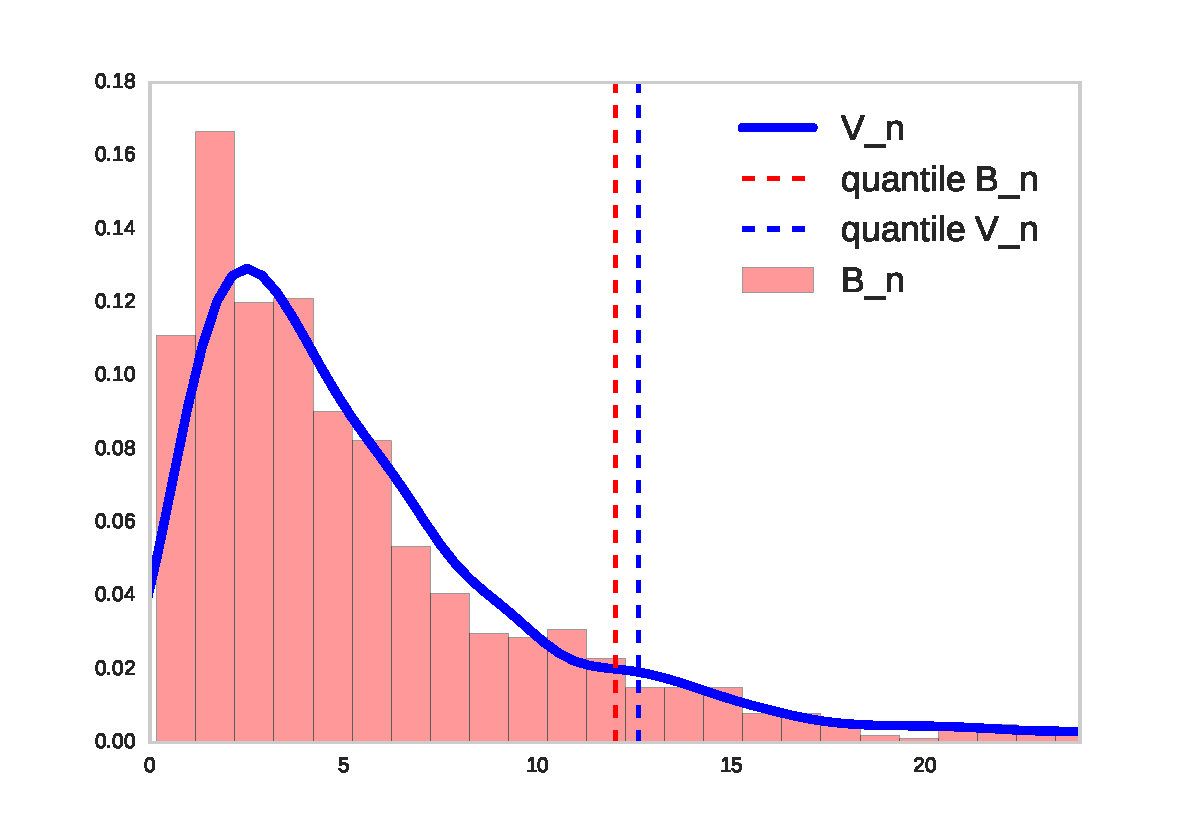
\includegraphics[width=\textwidth]{../../presentation/img/bootstrapWorks7.pdf}
 \caption{Brobdingnagian correlation in $W_t$} 
\end{figure}
  \end{minipage}
\begin{minipage}{.49\linewidth}
\begin{align*}
 X_t =& \beta X_{t-1} + \sqrt{1 - \beta^2}\epsilon_t\\
 & \epsilon_t \sim {\cal N}(0,1)
\end{align*}
 where $\beta$ controls the amount of autocorrelation in the process
\end{minipage}
\end{center}

 See also \cite{leucht_dependent_2013}.
\end{block}
\end{column}


% column 3
\hspace{-1.45cm}


\begin{column}{.32\linewidth}
%\vspace{-0.75cm}
\begin{block}{Consistency}
\large
 Suppose  $h$ is Lipschitz continuous and
$\ev h_{{ \color{red} p}}({ \color{blue} Z},{ \color{blue} Z})<\infty$. Under the null hypothesis $nV_n$ and $nB_n$ have the same limiting distribution (in a weak sense). Under the alternative hypothesis,
$B_{n}$ converges to zero, while $V_{n}$ converges to a positive
constant.

\end{block}


\vspace{-0.75cm}
\begin{block}{Experiment: Student's T vs.\ Normal}

\begin{center}
\begin{minipage}{.45\linewidth}
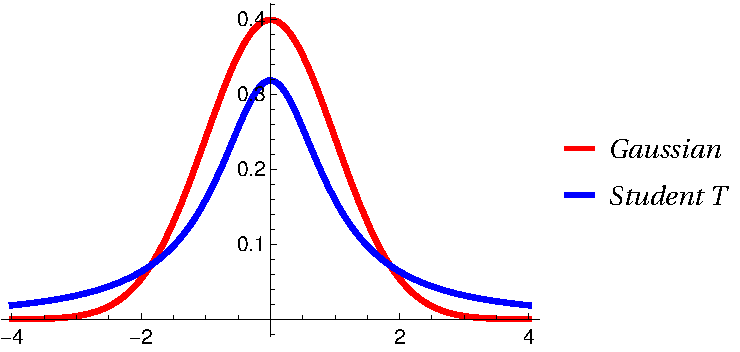
\includegraphics[width=\textwidth]{../../presentation/img/nt}
\end{minipage}
\begin{minipage}{.45\linewidth}
 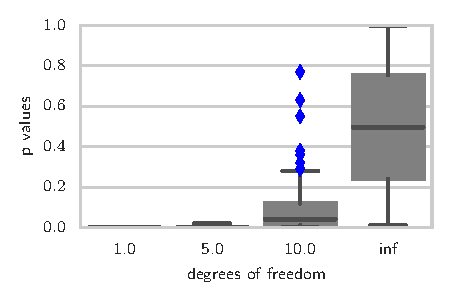
\includegraphics[width=\textwidth]{../../presentation/img/sgld_student_opt} 
\end{minipage}
\end{center}



We modify an experiment on comparing two densities from \cite{gorham2015measuring}. Our samples are non-iid and are generated using a random walk Metropolis algorithm.  We thin the observations by a factor of 20 and
set $a_{n}=0.1$. Our test both attains good statistical test power and
correct calibration of p-values under the null hypothesis.

\end{block}
\vspace{-0.75cm}


\begin{block}{Experiment: Bias quantification in Approximate MCMC}

 We  illustrate how to quantify bias-variance trade-offs in the (approximate) MCMC algorithm `austerity MCMC' \cite{korattikara2013austerity} on a simple generative model.

\begin{minipage}{.45\linewidth}
\begin{align*}
\theta_{1}\sim{\cal N}(0,10)\quad\theta_{2}\sim{\cal N}(0,1)\\\\
X_{i}\sim\frac{1}{2}{\cal N}(\theta_{1},4)+\frac{1}{2}{\cal N}(\theta_{1}+\theta_{2},4) & .
\end{align*}
\end{minipage}
\begin{minipage}{.45\linewidth}
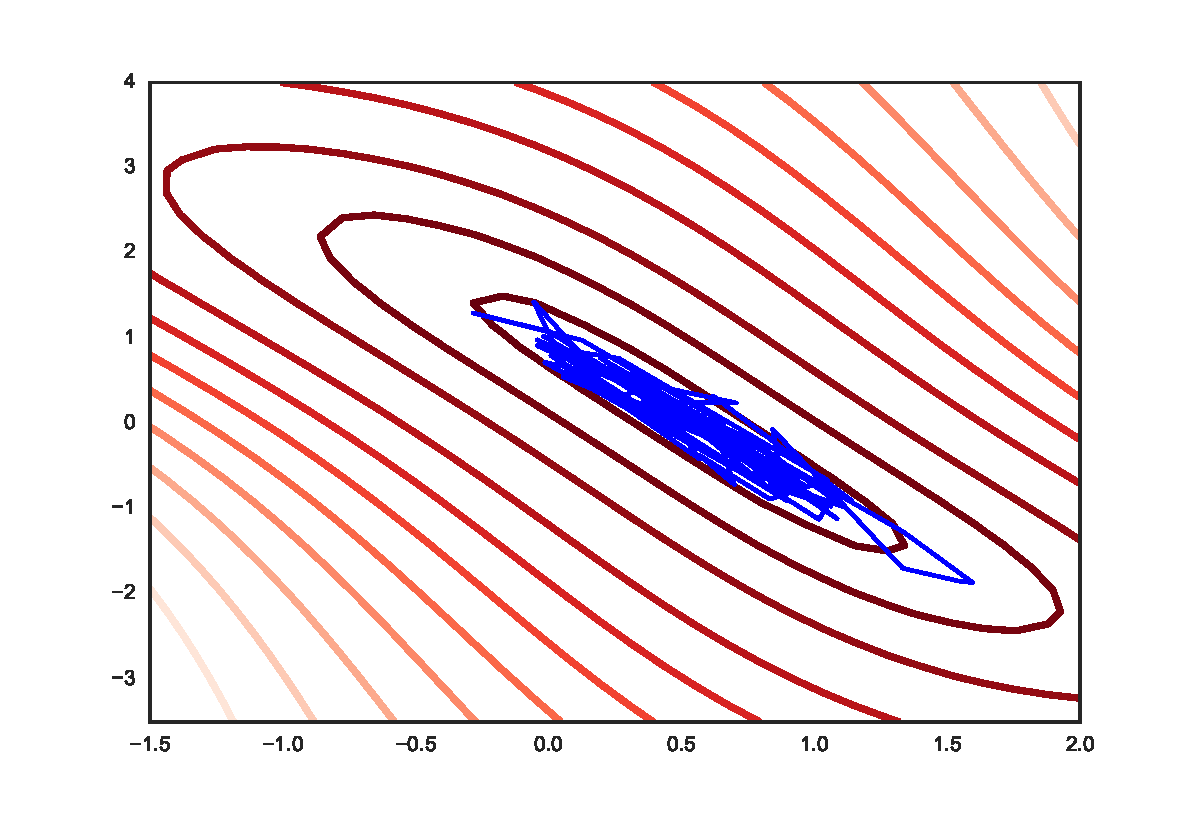
\includegraphics[width=\textwidth]{../../presentation/img/sgld_trace_and_density.pdf}
\end{minipage}


\footnotesize
Austerity MCMC is designed to reduce the number
of likelihood evaluation. The crux of method is to look at only a subset of the data,
and make an acceptance/rejection decision based on this subset. The
probability of making a wrong decision is proportional to a parameter
$\epsilon\in[0,1]$. We simulate $\{X_{i}\}_{1\leq i\leq400}$ points from the model
with $\theta_{1}=0$ and $\theta_{2}=1$. We run the algorithm with $\epsilon$ varying
over the range $[0.001,0.2]$. For each $\epsilon$ we calculate an
individual thinning factor, such that correlation between consecutive
 samples from the chains is smaller than $0.5$. For each $\epsilon$ we test the
hypothesis that $\{\theta_{i}\}_{1\leq i\leq500}$ is drawn from the
true stationary posterior, using our goodness of fit test. We generate
100 p-values for each $\epsilon$.


\begin{center}
\begin{minipage}{.450\linewidth}
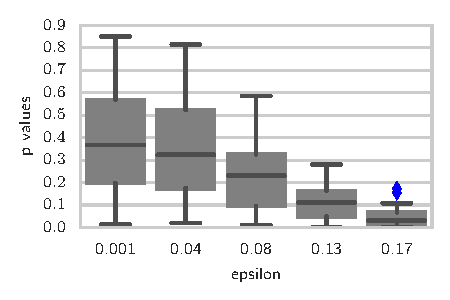
\includegraphics[width=\textwidth]{../../presentation/img/Heiko1}\\
\end{minipage}
\begin{minipage}{.45\linewidth}
            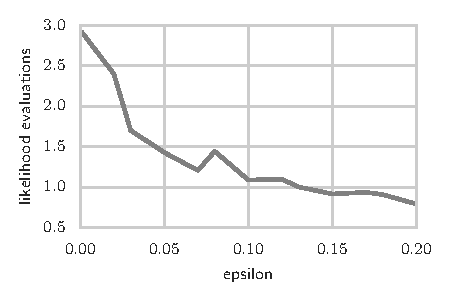
\includegraphics[width=\textwidth]{../../presentation/img/Heiko2}
\end{minipage}
\end{center}


\end{block}
\vspace{-0.75cm}
\begin{block}{Experiment: Statistical model criticism}
We test the hypothesis that a Gaussian process generated \textbf{training data}, previously using for fitting -- without simulating from the generative model, but only using {\color{red} test data}. This is in contrast to the test in \cite{lloyd2015statistical} that relies on sgenerative models.
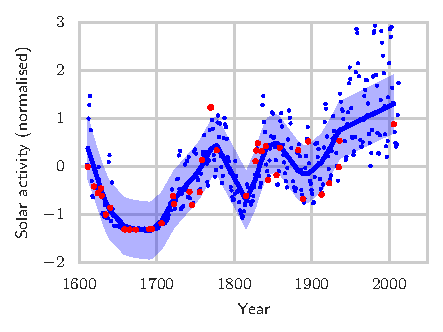
\includegraphics[width=0.48\textwidth]{../../presentation/img/gp_regression_data_fit.pdf} 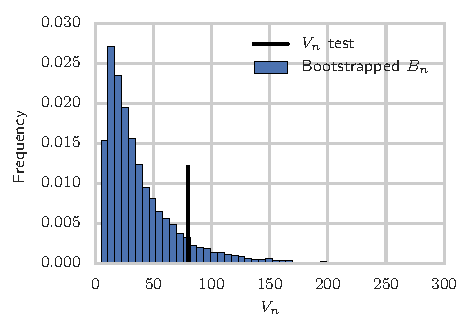
\includegraphics[width=0.48\textwidth]{../../presentation/img/gp_regression_bootstrap_hist} 
\begin{minipage}{.35\linewidth}

\end{minipage}
\end{block}

\vspace{-0.75cm}

\begin{block}{Experiment: Convergence in nonparametric density estimation}

 

We apply our goodness of fit test to measuring quality-of-fit in nonparametric density estimation. We evaluate two
density models: the infinite dimensional exponential family \cite{SriFukKumGreHyv14}, and a  approximation to this model \cite{strathmann2015gradient}.
% 

\begin{center}
\begin{minipage}{.450\linewidth}
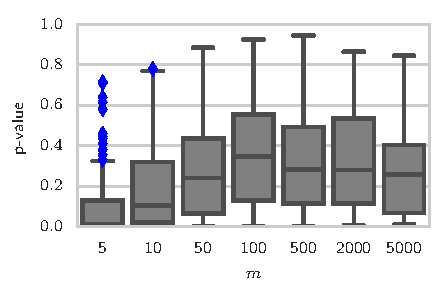
\includegraphics[width=\textwidth]{../../presentation/img/increasing_features_fixed_test}\\
\end{minipage}
\begin{minipage}{.45\linewidth}
            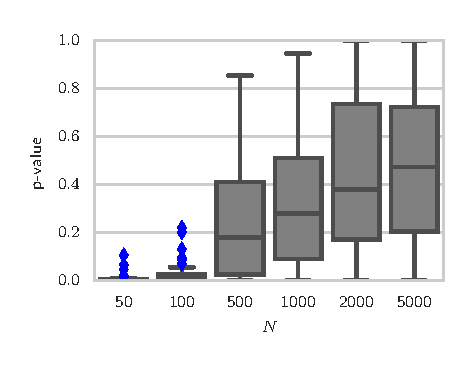
\includegraphics[width=\textwidth]{../../presentation/img/increasing_data_fixed_test}
\end{minipage}
\end{center}

\footnotesize
Our implementation of the model assumes
the log density to take the form $f(x)$, where $f$ lies in a RKHS
induced by a Gaussian kernel with bandwidth $1$. We fit the model
using $N$ observations drawn from a standard Gaussian, and perform
our quadratic time test on a separate evaluation dataset of fixed
size $n=500$. Our goal is to identify $N$ sufficiently large that
the goodness of fit test does not reject the null hypothesis.

\end{block}


\vspace{-0.75cm}
\begin{block}{References}


\begin{minipage}{.9\linewidth}
{\footnotesize
\begin{multicols}{2}
\setbeamertemplate{bibliography item}[text] 
\bibliographystyle{plain} 
\scriptsize
\bibliography{../../biblio.bib} \ 
\end{multicols}
} 
\end{minipage}
\end{block}

\end{column}
\end{columns}

\end{frame}
\end{document}
